\documentclass[tikz, border=3mm]{standalone}
\usepackage{tikz}
\usepackage{amsmath} % For \operatorname if needed, though not here
\usepackage{amssymb} % For \mathbb
\usetikzlibrary{positioning} % <<< Added this library

\begin{document}
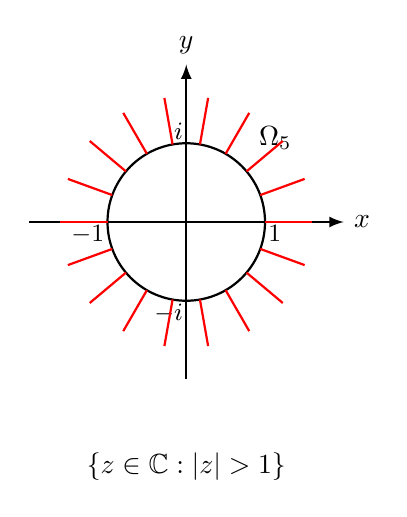
\begin{tikzpicture}[
    % Define axis style
    axis/.style={->, >=latex, thick},
    labelpos/.style={font=\small, inner sep=1pt} % Style for axis intercept labels
]

% Define radius and outer extent for hatching
\def\radius{1}
\def\outer{2} % How far the hatching lines should extend

% Axes
\draw[axis] (-\outer, 0) -- (\outer, 0) node[right] {$x$};
\draw[axis] (0, -\outer) -- (0, \outer) node[above] {$y$};

% Circle
\draw[thick] (0,0) circle (\radius);

% Axis Intercept Labels
\node[labelpos, below right] at (\radius, 0) {$1$};
\node[labelpos, below left]  at (-\radius, 0) {$-1$};
\node[labelpos, above left]  at (0, \radius) {$i$};
\node[labelpos, below left]  at (0, -\radius) {$-i$};

% Region Label
\node[above right] at (\radius*0.8, \radius*0.8) {$\Omega_5$};

% Hatching Lines (approximating the sketch)
\foreach \angle in {0, 20, 40, ..., 340} {
    % Draw slightly curved lines radiating outwards
    \draw[red, thick, bend left=5] (\angle:\radius) -- (\angle:\outer*0.8);
}

% Mathematical Description Below
% Give the origin node a name to position relative to it
\coordinate (origin) at (0,0);
% Now use the positioning library syntax correctly
\node[below=0.8cm of origin, yshift=-\outer cm] {$\{z \in \mathbb{C} : |z| > 1\}$}; % Position below origin, then shift down further

\end{tikzpicture}
\end{document}